\documentclass[final,t]{beamer}
\mode<presentation>
{
%  \usetheme{Warsaw}
%  \usetheme{Aachen}
%  \usetheme{Oldi6}
%  \usetheme{I6td}
  \usetheme{I6dv}
%  \usetheme{I6pd}
%  \usetheme{I6pd2}
}
% additional settings
\setbeamerfont{itemize}{size=\normalsize}
\setbeamerfont{itemize/enumerate body}{size=\normalsize}
\setbeamerfont{itemize/enumerate subbody}{size=\normalsize}
% additional packages
\usepackage{ragged2e}
\usepackage{verbatim}
\usepackage{textcomp}
\usepackage[ampersand]{easylist}
\usepackage{lipsum}
\usepackage{times}
\usepackage{amsmath,amsthm, amssymb, latexsym}
\usepackage{exscale}
%\boldmath
\usepackage{booktabs, array}
%\usepackage{rotating} %sideways environment
\usepackage[english]{babel}
\usepackage[latin1]{inputenc}
\usepackage[orientation=landscape,size=custom,width=111.76,height=86.36,scale=1]{beamerposter}
\addtobeamertemplate{block begin}{}{\justifying}
\usepackage[export]{adjustbox}
\listfiles
\graphicspath{{figures/}}
% Display a grid to help align images
%\beamertemplategridbackground[1cm]

\title{\huge YAX: Taxonomic assignment using metagenomic shotgun sequences}
\author{Evan T. Bolyen$^{a}$, Mike R. DeBerg$^{a}$, Andrew J. Hodel$^{a}$, Hayden T. Westbrook$^{a}$, and Viacheslav Y. Fofanov$^{a}$}
\institute{$^{a}$School of Computing, Informatics, and Cybersystems - Northern Arizona Univ.}

% abbreviations
\usepackage{xspace}
\makeatletter
\DeclareRobustCommand\onedot{\futurelet\@let@token\@onedot}
\def\@onedot{\ifx\@let@token.\else.\null\fi\xspace}
\def\eg{{e.g}\onedot} \def\Eg{{E.g}\onedot}
\def\ie{{i.e}\onedot} \def\Ie{{I.e}\onedot}
\def\cf{{c.f}\onedot} \def\Cf{{C.f}\onedot}
\def\etc{{etc}\onedot}
\def\vs{{vs}\onedot}
\def\wrt{w.r.t\onedot}
\def\dof{d.o.f\onedot}
\def\etal{{et al}\onedot}
\makeatother

%%%%%%%%%%%%%%%%%%%%%%%%%%%%%%%%%%%%%%%%%%%%%%%%%%%%%%%%%%%%%%%%%%%%%%%%%%%%%%%%%%%%%%%%%%%%%%%%%%%%%%%%%%%%
%%%%%%%%%%%%%%%%%%%%%%%%%%%%%%%%%%%%%%%%%%%%%%%%%%%%%%%%%%%%%%%%%%%%%%%%%%%%%%%%%%%%%%%%%%%%%%%%%%%%%%%%%%%%
\begin{document}
\begin{frame}{}
  \begin{columns}[t]
    \begin{column}{.3\linewidth}
        \begin{alertblock}{
\includegraphics[width=.9\linewidth]{assets/yak}\newline\newline}
            We introduce a novel pipeline called YAX which is used to assign taxonomy to provided samples. Whether it is a sample of dirt, subway grime, or your own gut, YAX will help to identify members of the community using high throughput metagenomic shotgun sequences.
          \newline
        \end{alertblock}
        \begin{block}{Intended Audience}
            \textbf{Features for Biologists:}
            \begin{itemize}
                \item[$\bullet$]Pipeline configuration based on textual input file
                \item[$\bullet$]Pipeline run recieves user input in text format
                \item[$\bullet$]Easy to understand error messages
                \item[$\bullet$]Parameter validation accomplished upon submission
                \item[$\bullet$]Dependency verification checks locations before run
            \end{itemize}
            \vspace{1cm}
            \textbf{Features for Bioinformatics Developers:}
            \begin{itemize}
                \item[$\bullet$]Modular design allows for pipeline reconfiguration
                \item[$\bullet$]Basic taxonomic tools included
            \end{itemize}
        \end{block}

        \begin{block}{Requirements}
            \textbf{Modular}
            \begin{itemize}
                \item[$\bullet$]Incorporate developing technologies
                \item[$\bullet$]Evaluate different processes
            \end{itemize}
            \vspace{1cm}
            \textbf{Fail Early}
            \begin{itemize}
                \item[$\bullet$]Validate parameters before running
                \item[$\bullet$]Verify dependencies before running
                \item[$\bullet$]Prevent failure in the middle of a run for spurious reasons
            \end{itemize}
            \vspace{1cm}
            \textbf{Coverage Representation}
            \begin{itemize}
                \item[$\bullet$]Provide biologists with relevant details
                \item[$\bullet$]Every identified taxon is qualified with coverage data
            \end{itemize}
            \vspace{1cm}
            \textbf{State System}
            \begin{itemize}
                \item[$\bullet$]Manage component requirements
                \item[$\bullet$]Control and record all data produced
                \item[$\bullet$]Eliminates redundant recomputation
                \item[$\bullet$]Allows parameter exploration
            \end{itemize}
        \end{block}



      %%%%%%%%%%%%%%%%%%%%%%%%%%%%%%%%%%%%%%%%%%%%%%%%%%%%%%%%%%%%%%%%%%%%%%%%%%%%%%%%%%%%%%%%%%%%%%%%%%%%%%%%%%%%


    \end{column}
    \begin{column}{.3\linewidth}
        %%%%%%%%%%%%%%%%%%%%%%%%%%%%%%%%%%%%%%%%%%%%%%%%%%%%%%%%%%%%%%%%%%%%%%%%%%%%%%%%%%%%%%%%%%%%%%%%%%%%%%%%%%%%
        \begin{block}{Purpose}
            To provide a dynamic solution to the process of taxonomic assignment. Rather than relying on one single purposed solution
            YAX relies on configration files to not only describe a single run of the tool but to describe the pipeline itself. In this
            way altering YAX to use slightly procesess is a trivial matter of developing an Artifact type and Module then including this
            module in the architectural configuration when bootstrapping the YAX State System. In intention of the current configuration
            of the YAX pipeline is to present the Biologist with data rather than conclusions. By offering as much releveant, qualifying
            data as possible the expertise of the biologist can be leverage rather than relying on an automated process.
        \end{block}

        \begin{block}{Solution Overview}
            Just need some words in between \\
            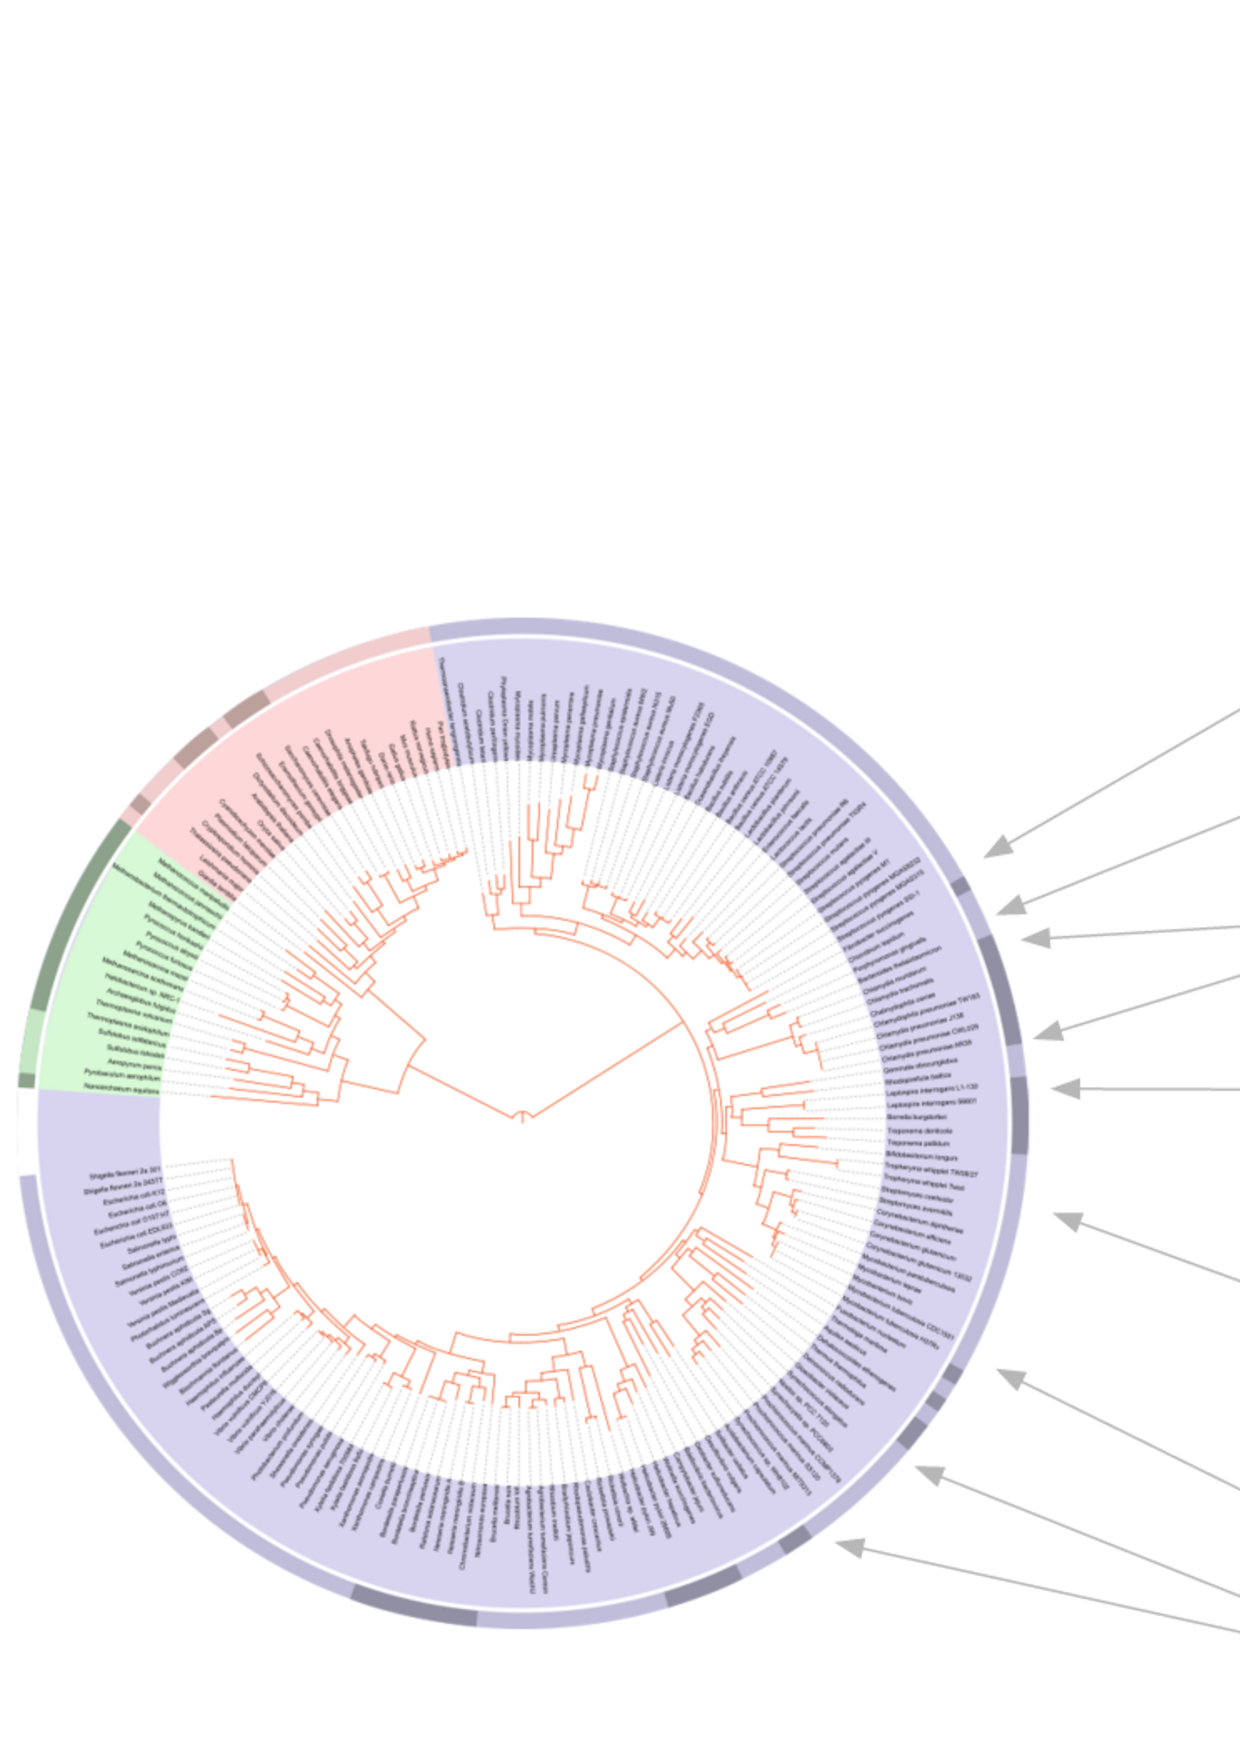
\includegraphics[width=1\linewidth]{assets/Whole} \\
            Some other words \\
            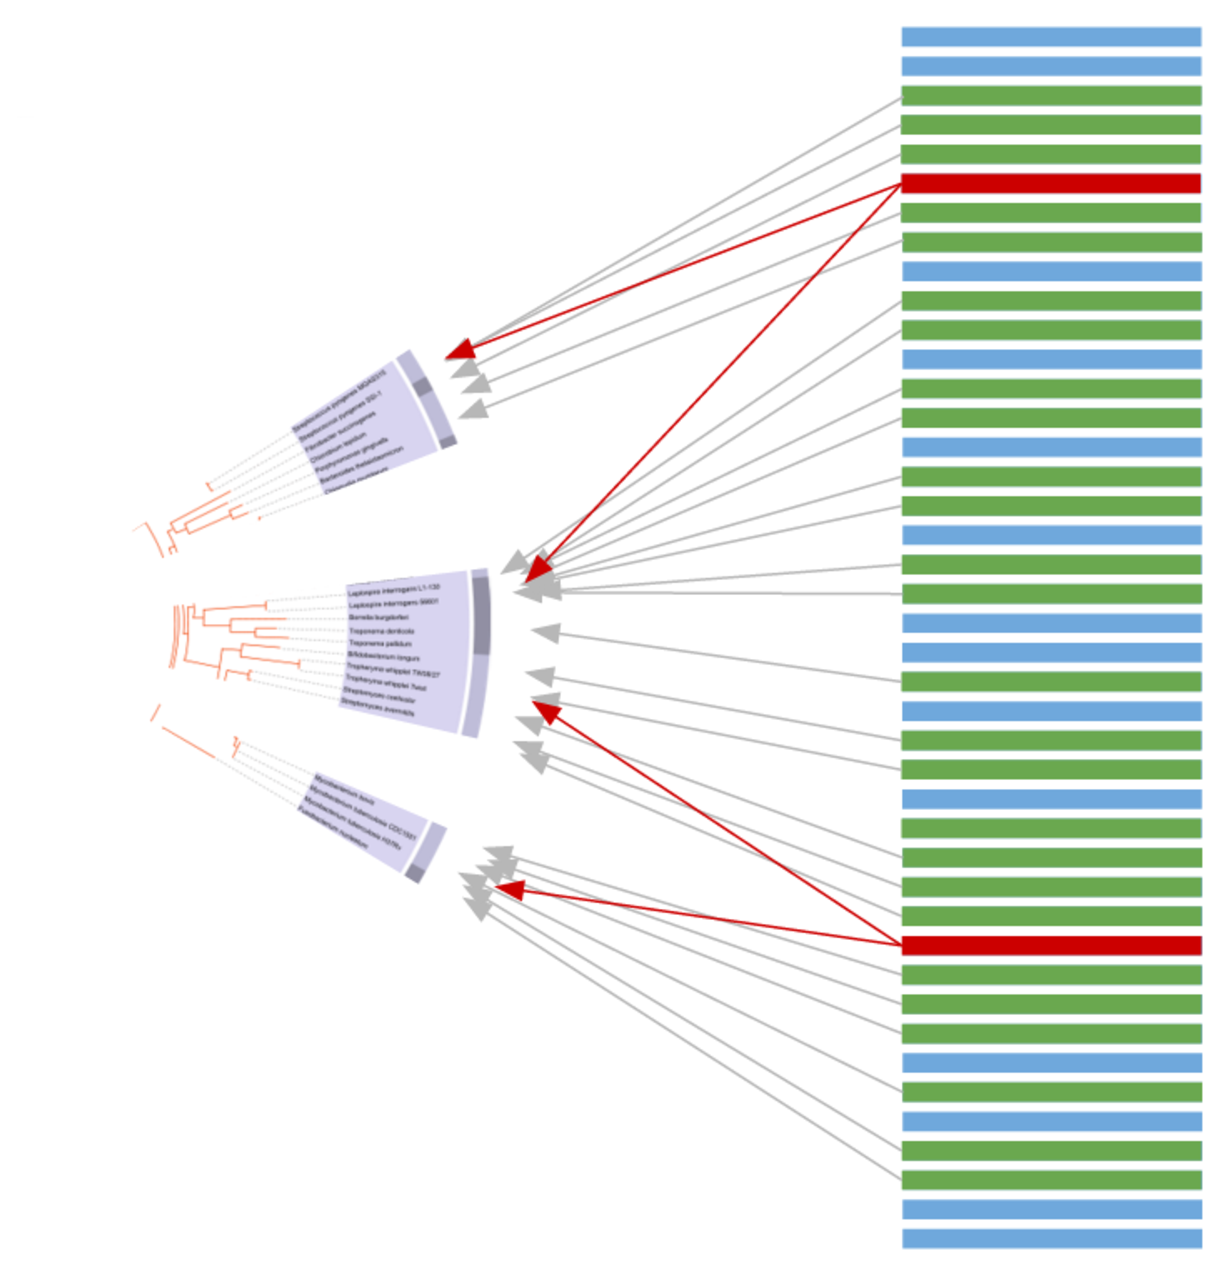
\includegraphics[width=0.679\linewidth, right]{assets/Subset}
        \end{block}


    \end{column}

    %%%%%%%%%%%%%%%%%%%%%%%%%%%%%%%

    \begin{column}{.3\linewidth}
        \begin{block}{Architecture}
            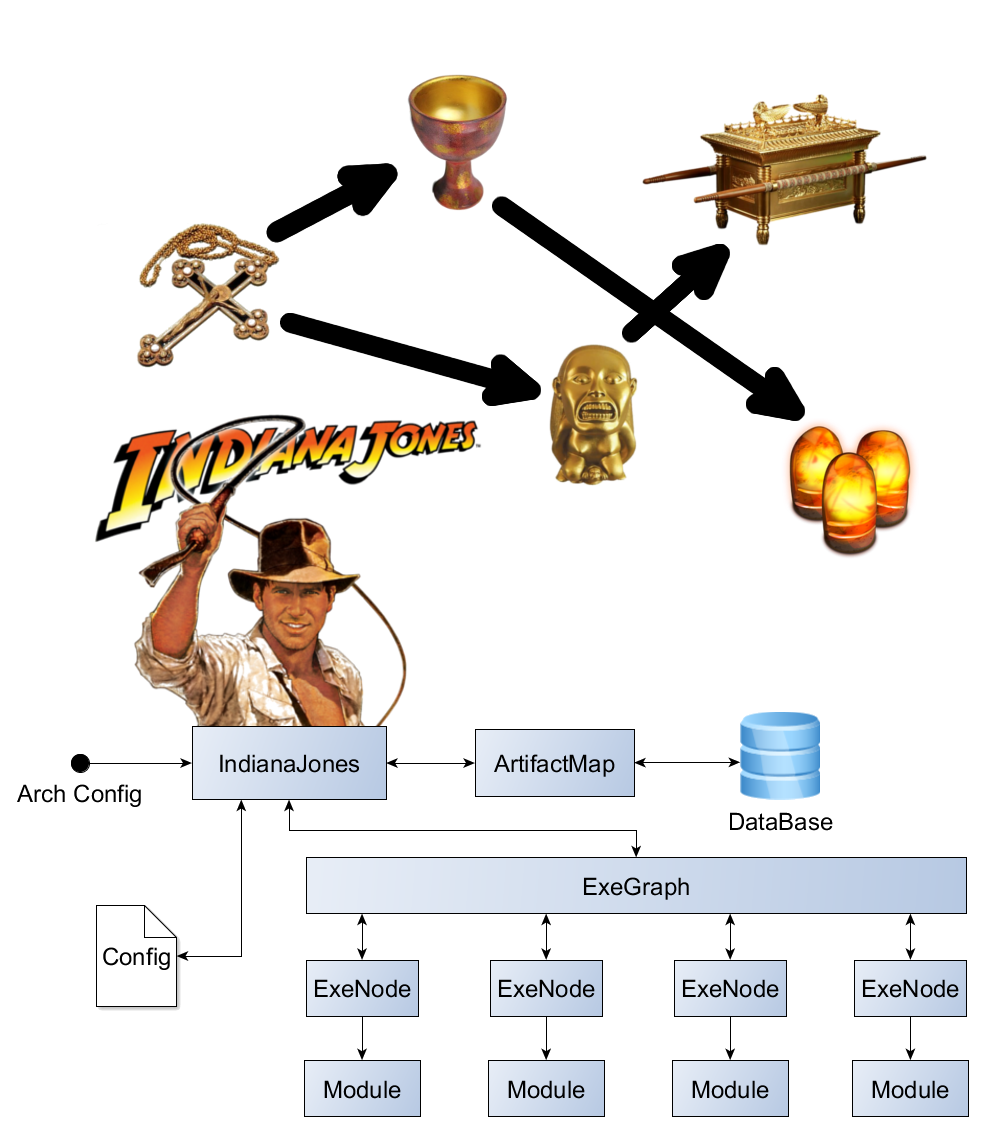
\includegraphics[width=1\linewidth]{assets/arch}\newline\newline

        \end{block}
        \begin{block}{Key Features}

        \end{block}



        \begin{block}{Future Work}
            YAX is designed to be highly modular and capable of adapting along side technological developments. As part of its development
            YAX was built to not only provide one solution but to investigate a number of possible solutions. The near future of YAX will
            see new modules developed to make fool use of its flexibility.

        \end{block}
        \begin{block}{References}
            \begin{itemize}
              {\small
              \item[1]Stack Overflow.
              \item[2]Bowtie2
              }
          \end{itemize}
        \end{block}

        %%%%%%%%%%%%%%%%%%%%%%%%%%%%%%%%%%%%%%%%%%%%%%%%%%%%%%%%%%%%%%%%%%%%%%%%%%%%%%%%%%%%%%%%%%%%%%%%%%%%%%%%%%%%



%%%%%%%%%%%%%%%%%%%%%%%%%%%%%%%%%%%%%%%%%%%%%%%%%%%%%%%

    \end{column}
  \end{columns}

\end{frame}

\end{document}


%%%%%%%%%%%%%%%%%%%%%%%%%%%%%%%%%%%%%%%%%%%%%%%%%%%%%%%%%%%%%%%%%%%%%%%%%%%%%%%%%%%%%%%%%%%%%%%%%%%%
%%% Local Variables:
%%% mode: latex
%%% TeX-PDF-mode: t
%%% End:
